\chapter{Covering spaces}\label{chapter:covering.spaces}

\section{Covering maps}
A continuous map \(f \colon X \to Y\) of topological spaces \emph{evenly covers}\define{evenly covered}
an open set \(U_Y \subset Y\) if \(f^{-1}U_Y \subset X\) is a disjoint union of open sets mapped homeomorphically to \(U_Y\) by \(f\), called \emph{sheets}\define{sheet}.
The map \(f \colon X \to Y\) is a \emph{covering map}\define{covering map} if \(Y\) has an open cover by evenly covered open sets.
A \emph{covering space} of a topological space \(Y\) is a topological space \(X\) equipped with a covering map \(f \colon X \to Y\). 
Covering spaces are the main tool to calculate fundamental groups.
\begin{exampleAndImage}{3cm}
The map \(\theta \in \R{} \mapsto \pr{\cos \theta, \sin \theta} \in S^1\) is a covering map.
Every open set of \(S^1\) which is not all of \(S^1\) is evenly covered: use trigonometry to write out an angle \(\theta\) for each point of your open set, well defined and unique up to adding \(2\pi\) multiples.
The sheets correspond to the \(2\pi\) multiples.
\tcblower
\includegraphics[width=3cm]{circle-covering}
\end{exampleAndImage}
\begin{example}
The map \(e^{i \theta} \in S^1 \mapsto e^{i n \theta} \in S^1\) is an \(n\)-sheeted covering.
\end{example}
\begin{example}
The map \(x \in \R{n} \mapsto \pr{e^{ix_1}, e^{ix_2}, \dots e^{ix_n}}\) is a covering map of the \(n\)-dimensional torus \(T^n\defeq S^1 \times S^1 \times \dots \times S^1\).
\end{example}
\begin{example}
The map \(x \in S^2 \mapsto [x] \in \RP{2}\) taking a point to the line through that point is a 2-sheeted covering of the projective plane.
\end{example}
\begin{example}
Take a manifold \(M\).
Let \(\hat{M}\) be the set of pairs \((m,o)\) where \(m \in M\) and \(o\) is an orientation of \(T_m M\), i.e. a choice of oriented basis up to equivalence, with two bases equivalent if the change of basis matrix between them has positive determinant.
Then \(\hat{M} \to M\) is a 2-1 covering map.
If \(M\) is orientable, then \(\hat{M}\) is a disjoint union of two copies of \(M\) and the covering map is a homeomorphism on each copy.
If \(M\) is not orientable, then \(\hat{M}\) is connected.
\end{example}
\begin{problem}{covering.spaces:zero.three}
Let \(X\) be the open interval \((0,3) \subset \R{}\).
Let \(Y\) be the unit circle in the complex plane.
Prove that the map \(f \colon X \to Y\) given by \(f(x)=e^{2\pi ix}\) is not a covering map.
\end{problem}
\begin{answer}{covering.spaces:zero.three}
Suppose that \(U_Y \subset Y\) is an evenly covered open set near \(1 \in Y\).
Write each point of \(Y\) as \(w = u+iv \in Y\).
Then \(U_Y\) contains a connected open set near \(1 \in Y\), say the ``interval'' \(-\varepsilon < v < \varepsilon\).
Since \(U_Y\) is evenly covered, so is this ``interval''.
The preimage of this ``interval'' is a union of 4 open intervals: 
\[
(0,\delta) 
\cup (1-\delta,1+\delta)
\cup (2-\delta,2+\delta)
\cup (3-\delta,3)
\]
where 
\[
\delta = \frac{\sin^{-1} \varepsilon}{2 \pi}.
\]
Any sheet over our open set is homeomorphic so also path connected, so lies inside one of these 4 intervals.
But no open subset of the first interval maps onto our ``interval'' as the map takes on values \(u+iv\) with \(0 < v < \varepsilon\) there.
\end{answer}
\begin{exampleAndImage}{6.63cm}
In the complex plane \(\C{}\), the map \(z \in \C{}-\set{0} \mapsto z^3 \in \C{}-\set{0}\) is a covering map.
We like to pretend that we can draw every covering map as a picture of ``sheets'', but in this case the best picture we get is an immersed surface.
\tcblower
\documentclass[tikz]{standalone}
\begin{document}
\begin{tikzpicture}
\clip (-4.03,-7.22) rectangle (2.6,5.15);
\fill[gray!25] (-.8,-6.2) ellipse (3.2cm and 1cm);
\fill[white,draw=gray] (-.8,-6.2) ellipse (.08cm and .025cm);
\node at (0,0) {\includegraphics[width=8cm]{complex-cube-root-graph-3}};
\end{tikzpicture}
\end{document}
\end{exampleAndImage}
\begin{problem}{covering.spaces:define.sheetedness}
Prove that the number \(n\) of sheets (which might be \(\infty\)) above an evenly covered open set is constant along any path in \(Y\).
In particular, if \(Y\) is path connected, this number \(n\) is constant, and we say that the covering map is \(n\) to \(1\).
\end{problem}
The \emph{fiber}\define{fiber} of a map \(f \colon X \to Y\) over a point \(y_0 \in Y\) is the set \(f^{-1}\set{y_0}\), usually denoted \(X_{y_0}\).
\begin{problem}{covering.spaces:discrete.fiber}
Prove that \(X_{y_0} \subset X\) is discrete, i.e. has the discrete topology as a subset of \(X\).
\end{problem}
\begin{answer}{covering.spaces:discrete.fiber}
Pick an evenly covered open set \(U_{y_0} \subset Y\) containing \(y_0\).
Every point \(x_0 \in X_{y_0}\) lies in a sheet, say \(U_{x_0}\), over \(U_{y_0}\).
Take two distinct points \(x_0, x_1 \in X_{y_0}\).
The sheets \(U_{x_0}\) and \(U_{x_1}\) are disjoint so \(x_1\) is not in \(U_{x_0}\) and \(x_0\) is not in \(U_{x_1}\).
Hence \(X_{y_0} \cap U_{x_0} = \set{x_0}\).
Take any subset \(S \subset X_{y_0}\).
Then 
\[
S = X_{y_0} \cap \bigcup_{x \in S} U_{x} 
\]
is the intersection of \(X_{y_0}\) with an open subset 
\[
\bigcup_{x \in S} U_{x} \subset X,
\]
so is open inside \(X_{y_0}\).
\end{answer}
\begin{problem}{covering.spaces:Hausdorfficity}
Suppose that \(f \colon X \to Y\) is a covering map.
Prove \(X\) is Hausdorff if and only if \(Y\) is Hausdorff.
\end{problem}
\begin{answer}{covering.spaces:Hausdorfficity}
Suppose that \(Y\) is Hausdorff. 
Take distinct points \(x_1, x_2\) of \(X\).
Let \(y_1=f(x_1)\) and \(y_2=f(x_2)\).

Suppose that \(y_1 \ne y_2\).
Take disjoint open sets \(U_1, U_2 \subset Y\) so that \(y_1 \in U_1\) and \(y_2 \in U_2\).
Then \(f^{-1}U_1, f^{-1}U_2 \subset X\) are disjoint open sets so that \(x_1 \in f^{-1}U_1\) and \(x_2 \in f^{-1}U_2\).

Suppose that \(y_1 = y_2\).
Take an evenly covered open set \(U \subset Y\) containing \(y_1\).
Every point \(x_1 \in X_{y_0}\) lies in a sheet, say \(U_{x_1}\), over \(U\).
The sheets \(U_{x_1}\) and \(U_{x_2}\) are disjoint open sets.

Now instead suppose that \(X\) is Hausdorff.
Take distinct points \(y_1, y_2\) in \(Y\).
Take two points \(x_1, x_2\) in \(X\) so that \(y_1=f(x_1)\) and \(y_2=f(x_2)\).
Pick evenly covered open sets \(U_{y_1}\) and \(U_{y_2}\) around \(y_1\) and \(y_2\).
Pick disjoint open sets \(W_{x_1}\) and \(W_{x_2}\) around \(x_1\) and \(x_2\).
Let \(U_{x_1}=W_{x_1} \cap f^{-1} U_{y_1}\).
Then \(f\) is a homeomorphism of \(U_{x_1}\) to its image inside \(U_{y_1}\); call its image \(V_{y_1}\).
Similarly define \(V_{y_2}\).
Because \(f\) homeomorphically maps \(U_{x_1}\) to \(V_{y_1}\), \(V_{y_1}\) is an open set in \(Y\).
The sets \(V_{y_1}\) and \(V_{y_2}\) are disjoint since they are images of disjoint open sets in \(X\).
\end{answer}
\begin{problem}{covering.spaces:compact}
Prove that every proper local diffeomorphism \(f \colon P \to Q\) between manifolds without boundary, with \(Q\) connected, is a covering map.
\end{problem}
\begin{answer}{covering.spaces:compact}
Take a point \(q_0\in Q\).
Because \(f\) is proper, the fiber \(P_{q_0} \defeq f^{-1}\Set{q_0}\) is compact.
Because \(f\) is a local diffeomorphism, each point \(p_0 \in P_{q_0}\) lies in an open set \(U_{p_0} \subset P\) taken by \(f\) diffeomorphically to a neighborhood  \(U_{q_0} \subset Q\).
The set \(P_{q_0}\) intersects \(U_{p_0}\) in a set taken by \(f\) to \(\Set{q_0}\), so just the single point \(p_0\).
Therefore every point \(p_0 \in P_{q_0}\) lies an open set \(U_{p_0}\) containing only \(p_0\), so \(P_{q_0}\) is a discrete set of points.
Being compact, \(P_{q_0}\) is therefore a finite set of points, say
\[
P_{q_0} = \Set{p_1, p_2, \dots, p_n},
\]
with each point \(p_j\) lying in an open set \(U_{p_j}\) taken diffeomorphically to some open set 
\[
f\of{U_{p_j}} \subset Q
\]
around \(q_0\).
Since there are finitely many such open sets, their intersection is open; call it \(U_{q_0}\).
Then replace \(U_{p_j}\) by
\[
U_{p_j} \cap f^{-1}U_{q_0} 
\]
so we can arrange that \(f\) takes each of the open sets 
\[
U_{p_1}, U_{p_2}, \dots, U_{p_n}
\]
diffeomorphically to \(U_{q_0}\).
\end{answer}
\begin{theorem}[Fundamental theorem of algebra]\define{theorem!fundamental, of algebra}\define{algebra!fundamental theorem of}\define{fundamental!theorem of algebra}
Suppose that \(k\) is a field containing \(\R{}\) and of finite dimension as a real vector space.
Then \(k=\R{}\) or \(k=\C{}\), up to isomorphism.
In particular, the splitting field of any real or complex polynomial is \(\R{}\) or \(\C{}\), i.e. every complex polynomial in one variable splits into a product of linear factors over \(\C{}\).
\end{theorem}
\begin{proof}
Pick any inner product on the real vector space \(k\).
Take the unit sphere \(S \subset k\).
The map \(f \colon x \in S \mapsto x^2/|x^2| \in S\) is smooth.
Compute that
\[
f'(x)y=\frac{2x}{|x^2|}\pr{y-\ip{f(x)}{xy}x}.
\]
In particular, if \(f'(x)y=0\) then \(y\) is a scalar multiple of \(x\).
So for \(y\) tangent to \(S\), \(f'(x)y=0\) just when \(y=0\), i.e. \(f\) is a local diffeomorphism.
The sphere is compact, so \(f \colon S \to S\) is a covering map.
If \(f(x)=f(y)\), pick a real number \(\lambda > 0\) so that \(\lambda^2=|x^2|/|y^2|\).
Check that \((x-\lambda y)(x+\lambda y)=0\), so \(x=\pm \lambda y\), i.e. up to scaling \(x=\pm y\), so \(f \colon S \to S\) is 2-1.
But the sphere of dimension \(2\) or more is simply connected, so does not admit a covering map of degree \(2\) from a connected space.
So \(S\) is the \(0\)-dimensional or \(1\)-dimensional sphere, i.e. \(k=\R{}\) or \(k\) is a \(2\)-dimensional real algebra.
Suppose that \(k\) is \(2\)-dimensional.
Pick some \(y \in k\) nonzero.
Then \(y/|y|\) lies in the image of \(f\), i.e., for some \(x\) with \(|x|=1\), 
\[
\frac{x^2}{|x^2|}=\frac{y}{|y|}.
\]
So if we let
\[
\lambda = \sqrt{\frac{|y|}{|x^2|}},
\]
and replace \(x\) by \(\lambda x\), we find \(x^2=y\).
So every nonzero element of \(k\) has a square root, and so in particular, \(-1 \in \R{}\) has a square root in \(k\), so \(k\) contains \(\C{}\), and hence \(k=\C{}\).
Note that we could pick \(k\) to be the splitting field of any real or complex polynomial.
\end{proof}
\begin{exampleAndImage}{5cm}
The \emph{harmonic archipelago} is given by drawing the Hawaiian earring on the plane, and then raising up the plane to a hollow hill, of unit height, between each successive pair of rings, with diameter of each hill becoming successively smaller approaching zero.
The limits of the hilltops are not in the archipelago, so it is not compact.
We can continuously deform any loop, based at the limit point of those hills, around finitely many hills in finite time, but not around all of them, since a map from a compact set has compact image.
The fundamental group is very complicated.
The set of points to the right of some line in our picture is homeomorphic to disk, so identified with a disk in any connected covering space.
Every connected covering space is thus a homeomorphism.
Wild Topology, Creative Commons Attribution 4.0 International License.
\tcblower
\includegraphics[width=5cm]{ha}
\end{exampleAndImage}

\section{Quotients by group actions}
An \emph{action}%
\define{group!action}%
\define{action!group}
of a group \(\Gamma\) on a topological space \(X\) is a map associating to each \(g \in \Gamma\) a continuous map \(X \to X\) denoted \(x \mapsto gx\) or sometimes denoted \(x \mapsto g \cdot x\), so that \(g(hx)=(gh)x\) for any \(g, h \in \Gamma\) and \(x \in X\) and so that \(1x=x\) for any \(x \in X\).
The action is \emph{free}\define{free!group action}\define{action!group!free}\define{group!action!free} if for any \(x \in X\), the only \(g \in \Gamma\) for which \(gx=x\) is \(g=1\).
The action is a \emph{covering action}%
\define{covering!group action}%
\define{action!covering}%
\define{group! action!covering} 
if any \(x \in X\) lies in an open set \(U \subset X\) so that the only \(g \in \Gamma\) for which \(gU\) intersects \(U\) is \(g=1\).
A group action is \emph{proper}%
\define{proper!group action}%
\define{group!action!proper}%
\define{action!group!proper}
when any points \(x, y \in X\) lie in open sets \(U_x, U_y\) so that \(gU_x\) intersects \(U_y\) for only finitely many \(g \in \Gamma\).
The \emph{orbit}\define{orbit} of a point \(x \in X\) is the set \(\Gamma x\defeq \set{gx|g \in \Gamma}\).
The \emph{quotient space}%
\define{quotient!space}%
\define{space!quotient}
\(X/\Gamma\) of the group action is the set of orbits, with the \emph{quotient map} \(x \in X \mapsto \Gamma x \in X/\Gamma\).
\begin{problem}{covering.spaces:prop.disc.metric}
Suppose that \(X\) is a metric space and that \(\Gamma\) acts on \(X\) by isometries.
Prove that \(\Gamma\) acts on \(X\) as a covering action if and only if the action is free with discrete orbits.
\end{problem}
\begin{problem}{covering.spaces:not.proper.disc}
Take an invertible matrix \(A\) with at least one eigenvalue \(\lambda\) satisfying \(\lambda > 1\) and at least one eigenvalue \(\mu\) satisfying \(0 < \mu < 1\).
Let \(M\defeq \R{n}-\set{0}\) and let \(\Gamma\defeq\set{A^n|n \in \Z{}}\).
Show that the action of \(\Gamma\) on \(M\) has discrete orbits, but the quotient space is not Hausdorff.
\end{problem}
\begin{problem}{covering.spaces:compact.quot}
If a group \(\Gamma\) acts on a topological space \(X\) and
\(X\) contains a compact set intersecting every \(\Gamma\)-orbit, then \(\bar{X}\) is also compact.
\end{problem}
\begin{theorem}\label{theorem:quotient.properly.discont}
Take a group \(\Gamma\) acting on a topological space \(X\).
The quotient map \(X \to \bar{X}= X/\Gamma\) is a covering map just when the action is a covering action.
\end{theorem}
\begin{proof}
For each point \(x \in X\) pick some open set \(U_x \subset X\) containing \(x\) so that \(gU_x\) doesn't intersect \(U_x\) for any \(g \in \Gamma\) unless \(g=1\).
The image \(\bar{U}_x \subset \bar{X}\) has preimage in \(X\) precisely the union of the nonoverlapping translates \(gU_x\) for \(g \in \Gamma\).
The open sets in \(\bar{U}_x\) have preimages precisely the \(\Gamma\)-invariant open sets in the translates of \(U_x\), precisely one of which lies in \(U_x\).
Hence the quotient map restricted to \(U_x\) is a homeomorphism \(U_x \to \bar{U}_x\).
Each element of \(\Gamma\) interchanges the sheets.
Conversely, if the quotient map is a covering map, then evenly covered open sets have preimages precisely open sets \(U\) not intersecting their translates \(gU\).
\end{proof}
\begin{theorem}\label{theorem:inv.open.sets}
Take an action of a group \(\Gamma\) on a Hausdorff space \(X\).
The quotient space is Hausdorff just when any two points of \(X\) lie in disjoint \(\Gamma\)-invariant open sets.
\end{theorem}
\begin{proof}
Take two points \(\bar{x}\ne \bar{y} \in \bar{X}\) in the quotient space \(\bar{X}\defeq X/\Gamma\).
Take points \(x, y \in X\) mapping to them.
If \(\bar{x}, \bar{y}\) lie in disjoint open sets \(\bar{U}_{\bar{x}}, \bar{U}_{\bar{y}}\), then the preimages of these open sets are disjoint \(\Gamma\)-invariant open sets around \(x\) and \(y\).

Conversely, take any disjoint \(\Gamma\)-invariant open sets around \(x\) and \(y\), \(U_x, U_y\).
Let \(\bar{U}_{\bar{x}}, \bar{U}_{\bar{y}}\) be their images in \(\bar{X}\).
By \(\Gamma\)-invariance, the preimage of \(\bar{U}_{\bar{x}}\) is \(U_x\) so \(\bar{U}_{\bar{x}}\) is open and \(\bar{U}_{\bar{x}} \cap \bar{U}_{\bar{y}}\) has preimage \(U_x \cap U_y\) empty so is empty.
\end{proof}
\begin{theorem}\label{theorem:proper.action}
Any proper group action on any Hausdorff space has Hausdorff quotient space.
\end{theorem}
\begin{proof}
Surround points \(x, y \in X\) with open sets \(U_x, U_y\) so that \(gU_x\) is disjoint from \(U_y\) except for finitely many \(g \in \Gamma\), say \(g_1, g_2, \dots, g_n\).
Because \(X\) is Hausdorff, for each \(j\) we can take ``houses'': disjoint open sets \(V_j, W_j\) so that \(V_j \subset g_j U_x\) and \(W_j \subset U_y\) and \(g_j x_j \in U_j\) and \(y \in W_j\).
Replace \(U_x\) with
\[
\bigcap_j g_j^{-1} U_j
\]
and \(U_y\) with
\[
\bigcap_j W_j.
\]
The resulting sets \(U_x\) and \(U_y\) have all translates disjoint, i.e. \(x\) and \(y\) lie in disjoint invariant open sets.
\end{proof}
A group \(\Gamma\) acting on a metric space \(X\) acts \emph{by isometries}%
\define{action!group!by isometries}%
\define{isometry!action}%
\define{group!action!by isometries}
if \(x \mapsto gx\) is an isometry for all \(g \in \Gamma\), i.e. \(d(gx,gy)=d(x,y)\) for any points \(x,y\) and \(g \in \Gamma\).
\begin{theorem}\label{theorem:metric.quotient}
Take a group action on a metric space \(X\) by a group of isometries \(\Gamma\).
The following are equivalent:
\begin{enumerate}
\item
The orbits are closed.
\item
Any two points of \(X\) lie in disjoint \(\Gamma\)-invariant open sets.
\item
The quotient space is a metric space, under the quotient metric
\[
d(\bar{x},\bar{y})=\inf_{g \in \Gamma} d(gx,y),
\]
so that the metric space topology agrees with the quotient topology.
\end{enumerate}
\end{theorem}
\begin{proof}
The orbits are closed just when any point in any orbit lies at a positive minimum distance from some point in any other chosen orbit, which occurs just when the ``quotient metric'' expression \(d\) is a metric.

Suppose that the orbits are closed.
Then the balls around distinct points \(\bar{x},\bar{y} \in \bar{X}\) have as preimages in \(X\) some disjoint \(\Gamma\)-invariant open sets.

Suppose that any two points \(x \ne y \in X\) lie in disjoint \(\Gamma\)-invariant open sets \(U_x, U_y\).
It is clear that the expression \(d\) above is continuous on \(\bar{X} \times \bar{X}\), since any open set of real numbers has open preimage inside \(X \times X\).
Next we want to prove that \(d(\bar{x},\bar{y})=0\) just when \(\bar{x}=\bar{y}\).
If \(d(g_j x, y) \to 0\) for some \(g_j \in \Gamma\), then \(g_j x\) enters \(U_y\) for all but finitely many \(j\), and so \(U_x \cap U_y\) is not empty.

So \(d\) is a metric on \(\bar{X}\).
If \(x \in X\) maps to \(\bar{x} \in \bar{X}\) then the ball of radius \(r\) around each point \(\bar{x}\) has preimage precisely the set of points \(y \in X\) so that \(d(gy,x)<r\) for some \(g \in \Gamma\), i.e. just exactly the union of \(\Gamma\)-translates of the ball of radius \(r\) around \(x\).
Take an open set \(\bar{W} \subset \bar{X}\) around \(\bar{x}\).
Let \(W \subset X\) be its preimage.
Pick a radius \(r\) small enough that the ball of radius \(r\) around \(x\) lies inside \(W\).
Then so do all \(\Gamma\)-translates.
So the ball of radius \(r\) around \(\bar{x}\) lies in \(\bar{W}\).
\end{proof}
A \emph{locally isometric covering map} is a map of metric spaces \(X \to Y\) so that every point of \(Y\) lies in an open set \(\bar{U}\) evenly covered, say by disjoint open sets \(U_{\alpha} \subset X\) for which \(U_{\alpha} \to \bar{U}\) is an isometry.
\begin{theorem}
Take a free group action on a metric space \(X\) by a group of isometries \(\Gamma\) with discrete orbits.
Then the quotient map \(X \to X/\Gamma\) is a locally isometric covering map.
\end{theorem}
\begin{proof}
The quotient is a metric space by theorem~\vref{theorem:metric.quotient}.
Take a point \(x \in X\) mapping to a point \(\bar{x} \in \bar{X}\) and a ball \(B \subset \bar{X}\) about \(\bar{x}\) of radius \(r\) small enough that it is evenly covered by balls \(B_{\alpha} \to B\) so that \(gB_{\alpha}\) doesn't intersect \(B_{\alpha}\) unless \(g=1\).
Let \(B' \subset B\) be the ball of radius \(r/2\) about \(\bar{x}\).
Pick points \(y,z \in X\) in the same sheet \(B'_{\alpha}\) mapping to points \(\bar{y}, \bar{z}\) in \(B'\).
The orbits are closed, so we can pick a point \(gz\) to be the closest point to \(y\) in the orbit \(\Gamma z\).
So \(d(gz,y)\le d(z,y)<r/2\) so \(d(gz,x) < r\).
But then \(gB_{\alpha}\) intersects \(B_{\alpha}\).
So \(g=1\).
Hence \(z\) is the closest point to \(y\) mapping to \(\bar{z}\).
Therefore \(d(z,y)=d(\bar{z},\bar{y})\), for all \(z,y \in B'_{\alpha}\).
\end{proof}
\begin{example}
The torus \(T^n=\R{n}/\Z{n}\) is the quotient of the \(\R{n}\) by the free action of \(\Z{n}\) with discrete orbits.
Hence the torus is a metric space in the quotient topology, and \(\R{n} \to T^n\) is a locally isometric covering map, as are all of the following examples.
\end{example}
\begin{example}
The real projective plane \(\RP{2}\) is the quotient of the unit sphere \(S^2 \subset \R{3}\) by the covering action of \(\Gamma=\Set{\pm 1}\).
\end{example}
\begin{example}
The \emph{M\"obius strip}%
\define{Moebius strip@M\"obius strip}
is the quotient \(\R{2}/\Gamma\) by the covering action of rigid motions \(\Gamma\) of the plane generated by the transformation 
\[
(x,y) \mapsto (x+1,-y).
\]
It is covered by the cylinder, given as the quotient \(\R{2}/\Gamma_0\) by the subgroup \(\Gamma_0 \subset \Gamma\) generated by
\[
(x,y) \mapsto (x+2,y).
\]
\begin{center}
\begin{tikzpicture}[scale=0.15]
\MoebiusStrip{Only}{one}{side}
\end{tikzpicture}
\end{center}
\end{example}
\begin{example}
The \emph{Klein bottle}%
\define{Klein bottle} is the quotient \(\R{2}/\Gamma\) by the covering action of rigid motions \(\Gamma\) of the plane generated by the two transformations
\[
(x,y) \mapsto (x,y+1)
\]
and
\[
(x,y) \mapsto (x+1,-y).
\]
It is clearly covered by the M\"obius strip, and by the cylinder.
\includegraphicsinexample[width=6cm]{klein-bottle-two-views}
\end{example}

\section{Lifting}
\begin{lemma}\label{lemma:unique.covering}
Take a covering map \(f \colon X \to Y\) from a Hausdorff space \(X\).
Take a path connected space \(Z\) and continuous maps \(g_1, g_2 \colon Z \to X\) so that \(f \circ g_1 = f \circ g_2\).
If \(g_1\of{z_0}=g_2\of{z_0}\) for some point \(z_0 \in Z\) then \(g_1=g_2\).
\end{lemma}
\begin{proof}
Suppose that \(g_1(z)=g_2(z)\) at some point \(z \in Z\).
Let \(x=g_1(z)\) and \(y=f(z)\).
Take an open set \(U_Y \subset Y\) around \(y\) so that \(f^{-1}U_Y\) is a disjoint union of sheets.
Let \(U_X\) be the sheet containing \(x\).
Let
\[
\tilde{f} \defeq \left.f\right|_{U_X}.
\]
Let 
\[
U_Z\defeq g_1^{-1} U_X \cap g_2^{-1} U_X.
\]
Clearly \(z \in U_Z\).
Moreover 
\[
f \circ g_1 = f \circ g_2
\]
implies that on \(U_Z\),
\[
\tilde{f} \circ g_1 = \tilde{f} \circ g_2.
\]
But \(\tilde{f}\) is a diffeomorphism, so on \(U_Z\), \(g_1=g_2\).

The set \(E\) of points \(z \in Z\) at which \(g_1=g_2\) is not empty because \(z_0\) lies in \(E\).
But \(E\) is open, since it contains an open set \(U_Z\) around each of its points as above.
But \(E\) is also closed, because \(X\) is Hausdorff.
Any path in \(Z\) starting in \(E\) stays in \(E\), because the set of points at which it lies in \(E\) is both an open and a closed subset of \([0,1]\).
Since \(Z\) is path connected, \(E\) is all of \(Z\).
\end{proof}
\begin{proposition}\label{covering.spaces:lift.path}
Take a covering map \(f \colon X \to Y\) from a Hausdorff space \(X\).
Take a path \(y \colon [0,1] \to Y\), and a point \(x_0 \in X\) so that \(f\of{x_0}=y(0)\).
There is a unique path \(x \colon [0,1] \to X\) so that \(f \circ x=y\) and \(x(0)=x_0\), the \emph{lift}\define{lift} of the path \(y\).
\end{proposition}
\begin{proof}
Uniqueness follows from lemma~\vref{lemma:unique.covering}.
Near each point \(y \in Y\) there is an evenly covered open set \(U_Y \subset Y\), i.e. so that \(f^{-1}U_Y\) is a disjoint union of open sets (the ``sheets''), each mapped homeomorphically to \(U_Y\) by \(f\).
For example, picking \(y\) to be \(y_0\), we find \(x_0\) on precisely one of these sheets, call it \(U_X\), and we define 
\[
x(t)=\left.f\right|_{U_X}^{-1}(y(t))
\] 
on the largest interval \(0 \le t < \tau\) for which \(y(t)\) stays inside \(U_Y\).

Cover \([0,1]\) by open intervals \(I_a\) so that \(y(t)\) stays inside an evenly covered set \(U_a\) on each open interval \(I_a\).
By compactness, extract a finite cover, and therefore a finite collection of intervals \(0 \le t \le a_1, a_1 \le t \le a_2, \dots, a_{n-1} \le t \le 1\), so that on each one \(y(t)\) stays inside an evenly covered open set \(U_1, U_2, \dots U_n\).
Lift up \(y(t)\) by inverting \(f\) over each \(U_i\) one at a time.
\end{proof}
\begin{proposition}
Suppose that \(f \colon X \to Y\) is a covering map from a Hausdorff space, and \(F \colon [0,1] \times Z \to Y\) is a continuous map, written \(F_s(z)\defeq F(s,z)\), and that there is a continuous map \(\hat{F}_0 \colon Z \to X\) so that \(f \circ \hat{F}_0 = F_0\).
Then there is a unique map \(\hat{F} \colon [0,1] \times Z \to X\) so that \(f \circ \hat{F}=F\) and \(\hat{F}(0,z)=\hat{F}_0(z)\) for all \(z \in Z\), the \emph{lift} of the map \(F\).
\end{proposition}
\begin{proof}
For each \(z_0 \in Z\), lift the path \(F\of{s,z_0} \in Y\) to a path \(\hat{F}\of{s,z_0}\), and this defines \(\hat{F}\of{s,z_0}\).
We need to prove that \(\hat{F}\) is continuous.
This is a purely local problem, so it suffices to prove for a trivial covering map, a homeomorphism, for which is it obvious.
\end{proof}
\begin{lemma}
The morphism of fundamental groups \(f_* \colon \fundamentalGroup{X} \to \fundamentalGroup{Y}\) of a covering map \(f \colon X \to Y\) on a Hausdorff space \(X\) is injective.
Its image is the set of loops in \(Y\) (modulo homotopy) which lift to loops in \(X\).
\end{lemma}
\begin{proof}
The kernel of \(f_*\) consists of the homotopy classes of the loops \(x \colon [0,1] \to X\) so that \(f \circ x \colon [0,1] \to Y\) is homotopic to the trivial loop.
Lift that homotopy up to a homotopy of \(x\) to the trivial loop.
Given a loop \(y\) with homotopy class in the image, \(x\) is its lift, a loop.
\end{proof}
Take a covering \(f \colon X \to Y\) with points \(x_0 \in X\) and \(y_0\defeq f\of{x_0} \in Y\).
Denote the fiber as \(X_{y_0}\defeq f^{-1}\Set{y_0}\). 
Given any loop \(\ell\) based at \(y_0\), let \(\hat{\ell}\) be its lift, a curve in \(X\) starting at \(x_0\).
Suppose that we replace \(\ell\) by a homotopy of loops \(\ell_t\) based at \(y_0\).
That homotopy lifts to a homotopy of curves \(\hat{\ell}_t\), all starting at \(y_0\).
Since \(\ell_t\) ends at \(y_0\), all of those curves \(\hat{\ell}_t\) end at points of \(X_{y_0}\).
Looking at our picture of sheets, we see that \(X_{y_0}\) is a discrete set, i.e. any continuous map to \(X_{y_0}\) is constant.
By continuity, the map \(t \mapsto \hat{\ell}_t(1)\) is constant.
So the endpoint \(\hat{\ell}(1)\) doesn't change if we move \(\ell\) through a homotopy.
Therefore we have a well defined map
\[
\fundamentalGroup{Y,y_0} \mapsto X_{y_0}.
\]
Take any loop \(x\) based at \(x_0\) and consider the associated loop \(y=f \circ x\) based at \(y_0\).
The loop \(y*\ell\) starts at \(y_0\) and its lift is \(x*\hat{\ell}\), with the same endpoints as \(\hat{\ell}\).
Therefore our map descends to a map
\[
\fundamentalGroup{Y,y_0}/f_* \fundamentalGroup{X,x_0} \mapsto X_{y_0}.
\]
\begin{lemma}
If \(X\) and \(Y\) are path connected Hausdorff topological spaces and \(f \colon X \to Y\) is a covering map, then the \emph{endpoint} map
\[
\fundamentalGroup{Y,y_0}/f_* \fundamentalGroup{X,x_0} \mapsto X_{y_0}
\]
is bijective.
\end{lemma}
\begin{proof}
Take any two points \(x_0, x_1 \in X_{y_0}\) and connected a path \(x\).
Then the loop \(y = f \circ x\) lifts to \(x\), so the map takes \(y\) to \(x_1\).
\end{proof}
\begin{proposition}\label{proposition:lift.map}
Take a covering map \(f \colon X \to Y\) from a Hausdorff space and a map \(g \colon Z \to Y\) from a path connected and locally path connected topological space \(Z\), 
\[
\begin{tikzcd}
      & X \arrow[d] \\
Z \arrow[r] & Y 
\end{tikzcd}
\]
and points \(z_0 \in Z\), \(x_0 \in X\), \(y_0 \in Y\) so that \(y_0=f\of{x_0}=g\of{z_0}\).
Then there is a unique lift \(\hat{g} \colon Z \to X\) so that
\[
\begin{tikzcd}
      & X \arrow[d] \\
Z \arrow[r] \arrow[ur] & Y 
\end{tikzcd}
\]
i.e. a map so that \(f \circ \hat{g}=g\) and \(\hat{g}\of{z_0}=x_0\), if and only if 
\[
g_* \fundamentalGroup{Z,z_0} \subset f_* \fundamentalGroup{X,x_0}.
\] 
\end{proposition}
\begin{proof}
If \(\hat{g}\) exists then \(g_*=f_* \circ \hat{g}_*\) so the image of \(g_*\) lies in the image of \(f_*\).
Suppose that the image of \(g_*\) lies in the image of \(f_*\).
Take a path \(z\) in \(Z\) starting at \(z_0\).
Map it a path \(y\) in \(Y\) and lift to a path \(x\) in \(X\).
Then define \(\hat{g}(z)=x(1)\).
This is a map \(z \mapsto \hat{g}(z)\) defined on paths.
Lifting homotopy of paths, \(\hat{g}(z)\) is clearly defined on homotopy classes of paths: \(\hat{g}([z])\).
Take two paths \(z,z'\) with the same endpoints in \(Z\) and let \(y,y'\) and \(x,x'\) be the corresponding paths in \(Y\) and lifts to \(X\).
Then \([z]^{-1}[z']\) is a loop in \(Z\), mapping to the loop \([y]^{-1}[y']\) in \(Y\), which lifts to a loop in \(X\).
By uniqueness of lifts, this loop is \([x]^{-1}[x']\).
In other words, \(x\) and \(x'\) have the same endpoint, so \(\hat{g}([z])=\hat{g}([z'])\) is that end point.
So \(\hat{g}([z])\) depends only on the endpoint \(z_1=z(1)\) of a path \(z\): \(\hat{g}(z_1)\), i.e. \(\hat{g} \colon Z \to X\).
Invert the covering map \(f\) locally, in some evenly covered open set in \(Y\).
Pick a simply connected open set in \(Z\) mapping to that open set in \(Y\).
Then paths in that simply connected open set will stay in the domain of the local inverse of \(f\).
We see that \(\hat{g}\) and \(g\) are locally identified by that local inverse of \(f\), so \(\hat{g}\) is continuous.
\end{proof}
\begin{problem}{covering.spaces:logs}
Suppose that \(Z \subset \C{}\) is a domain in the complex plane and that \(g \colon Z \to \C{}\) is a complex analytic function defined in \(Z\).
A \emph{logarithm}\define{logarithm} for \(g(z)\) is a complex analytic function \(G \colon Z \to \C{}\) so that \(g(z)=e^{G(z)}\).
Prove that \(g(z)\) has a logarithm \(G(z)\) just when both of the following conditions are satisfied:
\begin{enumerate}
\item \(g(z) \ne 0\) for any \(z \in Z\) and
\item \(g\) takes every loop in \(Z\) to a null homotopic loop in \(\C{}-\set{0}\).
\end{enumerate}
\end{problem}
Suppose that \(f \colon X \to Y\) is a covering space over a path connected space \(Y\).
Take two points \(y_0, y_1 \in Y\).
Take a path \(y(t) \in Y\) from \(y_0\) to \(y_1\).
For each point \(x_0 \in X_{y_0}\), let \(x_{x_0}(t)\) be the lift of \(y(t)\) that satisfies \(x_{x_0}(0)=x_0\).
Let \(h \colon [0,1] \times X_{y_0} \to X\), \(h_t\of{x_0}\defeq x_{x_0}(t)\).
Since the lift \(x_{x_0}(t)\) is uniquely determined by the choice of \(x_0\), this map \(h\) is well defined.
By problem~\vref{problem:covering.spaces:discrete.fiber}, every fiber \(X_{y_0}\) has the discrete topology as a subset of \(X\).
Hence \(h\) is continuous simply because each path \(x_{x_0}(t)\) is continuous.
The map \(h_t \colon X_{y_0} \to X_{y_1}\) has inverse given by following the path \(y(t)\) backwards and constructing the same sort of map as \(h\).
In particular, the fibers \(X_{y_0}\) and \(X_{y_1}\) are homeomorphic via \(h_1 \colon X_{y_0} \to X_{y_1}\), the \emph{monodromy}\define{monodromy} of the path \(y(t)\).

By the homotopy lifting lemma, the monodromy depends only on the homotopy class of \(y(t)\), giving a group morphism from \(\fundamentalGroup{Y,y_0}\) to the group of permutations of the elements of \(X_{y_0}\), the \emph{monodromy morphism}.
\begin{problem}{covering.space:monodromy.proj.plane}
Let \(X\) be the unit sphere in \(\R{3}\), let \(Y\) be the projective plane, and let \(f \colon X \to Y\) be the usual covering map: \(f(x)\) being the line through the origin passing through \(x\).
Take the path \(x(t)=(\cos \pi t, \sin \pi t, 0) \in X\) and let \(y(t)=f(x(t))\).
Explain why \(y(t)\) is a loop and calculate its monodromy morphism.
\end{problem}
\begin{problem}{covering.space:monodromy.group.quotient}
Take a path connected Hausdorff space \(X\) with covering action of a group \(\Gamma\) and let \(\bar{X}=\Gamma\backslash X\).
Explain how to find the monodromy of the covering map \(x \in X \mapsto \Gamma x \in \bar{X}\) over any loop in \(\bar{X}\).
\end{problem}
\begin{problem}{covering.space:rptwo.to.torus}
Prove that every continuous map \(X \to Y\) from the real projective plane \(X\) to the 2-dimensional torus \(Y\) is null homotopic.
\end{problem}

\section{The universal covering space}
A \emph{universal covering space}%
\define{covering space!universal}%
\define{universal covering space}%
\define{space!universal covering}
of a topological space \(Y\) is a simply connected covering space \(X\) of \(Y\).
The map \(X \to Y\) is a \emph{universal covering map}.
\begin{example}
The map \(\theta \in \R{} \mapsto e^{i \theta} \in S^1\) is a universal covering map.
\end{example}
\begin{example}
The map \(x \in S^2 \to [x] \in \RP{2}\), taking a unit vector \(x\) to the line through \(0\) and \(x\), is a universal covering map.
\end{example}

A \emph{morphism}\define{morphism!of covering spaces}\define{covering space!morphism} of covering spaces \(X \to Y\) and \(Z \to Y\) is a continuous map \(X \to Z\) making a commutative diagram:
\DeltaCommutativeDiagram{X}{Y}{Z}
\begin{problem}{covering.spaces:cover.cover}
Prove that \(X \to Z\) is then also a covering map.
\end{problem}
\begin{problem}{covering.spaces:universal.property}
Suppose that \(Y\) is a Hausdorff topological space which admits a universal covering space.
Prove that a covering map \((X,x_0) \to (Y,y_0)\) is universal just when every other covering map \((Z,z_0) \to (Y,y_0)\) has a unique morphism \((X,x_0) \to (Z,z_0)\).
\end{problem}
\begin{answer}{covering.spaces:universal.property}
If \(X\) is a universal covering space, then the map \(X \to Y\) lifts to a map \(X \to Z\) by proposition~\vref{proposition:lift.map}.

Take a covering map \((X,x_0) \to (Y,y_0)\) so that every other covering map \((Z,z_0) \to (Y,y_0)\) has a unique covering map \((X,x_0) \to (Z,z_0)\) making a commutative diagram
\DeltaCommutativeDiagram{X}{Y}{Z}
Take a universal covering map \((Z,z_0) \to (Y,y_0)\).
Take the unique covering map described above.
Any loop in \(X\) maps into \(Z\), where it is homotopic to a constant map.
Map that homotopy into \(Y\), and then lift the curves of that homotopy up to curves in \(X\), which are loops by taking the ``endpoint of the lift'' mapping.
So then \(X\) is simply connected, i.e. a universal covering map.
\end{answer}
An \emph{isomorphism}\define{isomorphism!of covering spaces}\define{covering space!isomorphism}
is a morphism with an inverse morphism.
\begin{problem}{covering.spaces:unique.ucs}
Suppose that \(X_1 \to X\) and \(X_2 \to X\) are universal covering spaces of a Hausdorff space \(X\).
Pick points \(x_1 \in X_1\) and \(x_2 \in X_2\) mapping to the same point \(x_0 \in X\).
Prove that there is a unique isomorphism taking \(x_1\) to \(x_2\).
\end{problem}
\begin{answer}{covering.spaces:unique.ucs}
By problem~\vref{problem:covering.spaces:universal.property}, there are unique morphisms \((X_1,x_1) \to (X_2,x_2)\) and \((X_2,x_2) \to (X_1,x_1)\).
The composition of these a morphism \(X_1 \to X_1\). 
Again by problem~\vref{problem:covering.spaces:universal.property}, there is a unique such morphism.
But the identity map is a morphism.
So \(X_1 \to X_2\) composes with \(X_2 \to X_1\) to give the identity map.
Swapping the roles of \(X_1\) and \(X_2\), the same is true for the composition in the other order.
Therefore the two morphisms are inverses of each other.
\end{answer}
\begin{theorem}\label{theorem:existence.of.universal.cover}
Every path connected and locally simply connected topological space \(X\) has a universal covering space \(\tilde{X} \to X\).
\end{theorem}
\begin{proof}
Pick a point \(x_0 \in X\).
Let \(\tilde{X}\) be the set of all paths starting at \(x_0\), modulo homotopy fixing endpoints.
Let \(\tilde{x}_0=\left[1_{x_0}\right]\) be the homotopy class of the trivial loop.
Map \(p \colon [x] \in \tilde{X} \mapsto x(1) \in X\), a surjective map.
The open sets \(U \subset X\) which are simply connected form a basis of open sets on \(X\).
To such a set \(U\) and a path \(x\) from \(x_0\) to a \(x_1 \in U\), with homotopy class \([x]\) with fixed endpoints, we associate the set
\[
U_{[x]} \defeq \Set{[x*y]|\text{\(y\) is a path in \(U\) and \(y(0)=x(1)\)}} \subset \tilde{X}.
\]
Note that \([x] \in U_{[x]}\), so these sets \(U_{[x]}\) cover \(\tilde{X}\).
We take these sets \(U_{[x]}\) be a basis of open sets in \(\tilde{X}\).
Note that
\[
p\of{[x*y]}=y(1) \in U,
\] 
so that
\[
p\of{U_{[x]}}=U.
\]
Since \(U\) is simply connected, any two paths \(y, z\) from \(x(1)\) to \(y(1)=z(1)\) are homotopic, so \([x*y]=[x*z]\), i.e. \(p\) is injective on \(U_{[x]}\).
So \(p\) is a bijection 
\[
p \colon U_{[x]} \to U.
\]
If \([z] \in U_{[x]}\) then \([z]=[x*y]\) for some \(y\).
But then \([x]=[\bar{y} * z]\), so
\[
[x] \in U_{[z]}.
\]

Take any two such open sets \(U_{[x]}, V_{[y]}\), containing some common point \([z]\), we see than that 
\[
U_{[x]}=U_{[z]}
\]
and
\[
V_{[y]}=V_{[z]}.
\]
Take an open subset \(W \subset U \cap V\), connected and simply connected.
Then
\[
W_{[z]} \subset U_{[x]} \cap V_{[y]}.
\]
Therefore the sets \(U_{[x]}\) form the basis of a topology: their unions are closed under finite intersections.
Note that
\[
p^{-1}U = \bigcup_{[x]} U_{[x]}
\]
where the union is over all paths \(x\) from \(x_0\) to a point of \(U\).
The map \(p \colon \tilde{X} \to X\) is therefore continuous.

We want to show that the map
\[
\left.p\right|_{U_{[x]}} \colon U_{[x]} \to U
\]
has a continuous inverse.
This is a bijection, so has an inverse, call it \(q\).
We need only check that, for any open set of \(U_{[x]}\), the inverse image via \(q\) is also open.
In other words, we need only check that, for any open set of \(U_{[x]}\), the image via \(p\) is also open.
Since the various \(\set{W_{[y]}}\) open sets form a basis for our topology, it is enough to check that, for any simply connected open set \(W \subset U\), and path \(y\) from \(x_0\) to a point of \(W\), the image
\[
p W_{[y]} \subset U
\]
is open.
But this is just exactly \(W\), since \(W\) is path connected, so every point of \(W\) is the endpoint of a path in \(W\).

Given any path \(x(t)\) starting at \(x_0\), let 
\[
x_s(t)
=
\begin{cases}
x(t), & \text{ if \(0 \le t \le s\)}, \\
x(s), & \text{ if \(s \le t \le 1\)}.
\end{cases}
\]
The homotopy class \(\left[x_t\right]\) is a path \(\tilde{x}(t)=\left[x_t\right]\) in \(\tilde{X}\) from \(\tilde{x}_0\) to \(\left[x_1\right]\).
So \(\tilde{X}\) is path connected.

Take a loop \(x(t)\) in \(X\) starting and ending at \(x_0\).
The loop lifts to a path \(\tilde{x}(t)\) as above.
By definition, the path \(\tilde{x}(t)\) is a loop just when \(\tilde{x}(1)=\tilde{x}(0)=\left[1_{x_0}\right]\).
But \(\tilde{x}(1)=\left[x_1\right]=\left[x\right]\) is the homotopy class of \(x\), so the lift is a loop just when the original loop is null homotopic, in which case the lift is null homotopic.
\end{proof}
\begin{problem}{covering.spaces:Rn}
Suppose that \(f \colon \R{n} \to \R{n}\) is a continuously differentiable map, that \(f'(x)\) is an invertible matrix for every \(x \in \R{n}\), and that, for any sequence \(x_1, x_2, \dots\) with \(\norm{x_i} \to \infty\), \(\norm{f\of{x_i}} \to \infty\).
Prove that \(f\) is a diffeomorphism.
\end{problem}
\begin{answer}{covering.spaces:Rn}
By hypothesis, for any point \(y_0 \in \R{n}\), the fiber \(f^{-1}\set{y_0}\) is bounded, but also closed, so compact.
But around each point \(x_0 \in f^{-1}\set{y_0}\), \(f\) is a local diffeomorphism, so \(x_0\) is isolated in \(f^{-1}\set{y_0}\).
So \(f^{-1}\set{y_0}\) is discrete and compact, so finite, say equal to \(\set{x_1,x_2,\dots,x_N}\).
Take a small enough open set around each \(x_i\) so that \(f\) is a diffeomorphism on that open set.
Inside each, take a compact set containing a neighborhood of \(x_i\), and take the images of those compact sets.
Because \(f\) is a local diffeomorphism, each of these images contains some relatively compact open neighborhood of \(y_0\).
So their intersection does as well.
But then that open neighborhood is evenly covered.
\end{answer}
The fundamental group \(\fundamentalGroup{X,x_0}\) acts on the universal covering space \(\tilde{X}\) by the action \([x][y]=[x*y]\), which is clearly continuous. 
The covering map \(\tilde{X} \to X\) is invariant under the action.
\begin{lemma}
Take a path connected and locally simply-connected topological space \(X\).
The action of the fundamental group on the universal covering space is a covering action.
\end{lemma}
\begin{proof}
We use the notation of theorem~\vref{theorem:existence.of.universal.cover}.
Take two points \(\left[x_1\right], \left[x_2\right] \in \tilde{X}\).
If the paths \(x_1(t)\), \(x_2(t)\) have distinct endpoints, say \(x_1(1) \ne x_2(1)\), then pick disjoint open sets \(U, W\) around them, and then \(U_{[x_1]}\) does not intersect \(W_{[x_2]}\).
If the paths have the same endpoint, take a simply connected open set \(U\) containing that endpoint: \(x_1(1)=x_2(1) \in U\).
If the open sets \(U_{[x_1]}\) and \(U_{[x_2]}\) are not disjoint, then they are equal (as we saw in the proof of theorem~\ref{theorem:existence.of.universal.cover}).
The homeomorphism \(p \colon U_{[x_1]} \to U\) over the evenly covered open sets \(U\) then identifies the points \([x_1], [x_2] \in \tilde{X}\), so the points of \(\tilde{X}\) are not distinct.
\end{proof}
\begin{problem}{covering.spaces:R.cov}
Prove that the only topological spaces with \(\R{}\) as a covering space are \(\R{}\) and \(S^1\).
\end{problem}
\begin{answer}{covering.spaces:R.cov}
Consider the fundamental group action, a covering group action on \(\R{}\).
Every orbit is discrete.
Pick some \(t_0\in\R{}\).
It has a discrete orbit: some \(t_i\in\R{}\), which we can write it order \(t_i<t_{i+1}\).
Each element of the group is uniquely determined by how it maps any one point, since they act without fixed points.
Define elements \(\gamma_i\) by \(\gamma_i(t_0)=t_i\).
Define a group operation on these \(t_i\), isomorphic to the fundamental group, by \(t_i+t_j=t_k\) if \(\gamma_j(\gamma_i(t_0))=\gamma_k(t_0)\).

Each element of the fundamental group is a homeomorphism of \(\R{}\), so an increasing or decreasing proper map \(\R{}\to\R{}\).
If decreasing, it has a fixed point by the intermediate value theorem, so it is an increasing function, so preserves the ordering of the \(t_i\).
Hence \(t_j\) takes \(t_0\mapsto t_0+t_j=t_j\), and so sends \(t_1\) to \(t_{j+1}\), and so on.
Hence the fundamental group is isomorphic to \(\Z{}\).
Each interval \([t_i,t_{i+1}]\) is mapped to the quotient space injectivity except at the ends, so quotients to \(S^1\), an bijective continuous map from a compact Hausdorff space, so a homeomorphism by theorem~\vref{theorem:continuous.bijection}.
\end{answer}
\begin{lemma}\label{lemma:covering.spaces.and.groups}
Take a path connected and locally simply connected space \(X\).
Every subgroup \(\Gamma \subset \fundamentalGroup{X}\) arises as the image of the fundamental group of a connected covering space \(X_{\Gamma} \to X\).
Any connected covering space \(Z \to X\) whose fundamental group has image \(\Gamma\) is isomorphic to \(X_{\Gamma} \to X\).
\end{lemma}
\begin{proof}
Let \(X_{\Gamma}\defeq \tilde{X}/\Gamma\), with the topology generated by declaring open sets to be the preimages of the open sets of \(X\) under the quotient map.
So \(\tilde{X} \to X_{\Gamma} \to X\) are continuous maps, and indeed covering maps.
Take a connected covering space \(f \colon Z \to X\) for which \(\fundamentalGroup{Z}\) maps to \(f_* \fundamentalGroup{Z} = \Gamma\).
By proposition~\vref{proposition:lift.map}, the map \(f \colon Z \to X\) lifts to a map \(\hat{f} \colon Z \to X_{\Gamma}\), and the covering map \(p \colon X_{\Gamma} \to X\) lifts to a map \(\hat{p} \colon X_{\Gamma} \to Z\).
We leave the reader to check that these maps are inverses of one another.
\end{proof}
\begin{corollary}\label{corollary:quotient.f.g}
If a group \(\Gamma\) has a covering action on a simply connected and locally simply connected Hausdorff topological space \(X\), then the quotient has fundamental group
\[
\fundamentalGroup{\Gamma\backslash X}=\Gamma
\]
and the quotient map \(X \to \Gamma\backslash X\) is the universal covering map.
\end{corollary}
\begin{example}
The fundamental group of the Klein\SubIndex{Klein bottle} bottle is the nonabelian group generated by the two transformations
\[
(x,y) \mapsto (x,y+1)
\]
and
\[
(x,y) \mapsto (x+1,-y)
\]
of the plane.
Picture how this acts on the \(1 \times 1\) squares with integer corners.
Since the \((x,y)\)-plane is the universal covering space of the Klein bottle, the preimage of each point is an orbit of these transformations.
Each element of the group is identified with such a point, so the group is identified with the integer points of the plane, but with a tricky group operation.
\end{example}
\begin{example}
The fundamental group of the torus \(\R{2}/\Z{2}\) is \(\Z{2}\), abelian.
Hence the Klein bottle is not homeomorphic to the torus.
\end{example}
\begin{example}\label{example:rpn.pi.1}
The fundamental group of \(\RP{n}\) is \(\pm 1\), from the covering map \(S^n \to \RP{n}\) and the fact that \(S^n\) is simply connected.
\end{example}

\section{Deck transformations}
A \emph{deck transformation}%
\define{deck transformation} 
of a covering map \(f \colon X \to Y\) is a homeomorphism \(g \colon X \to X\) so that \(f \circ g = f\).
\begin{example}
For any integer \(n\), the map \(\theta \mapsto \theta+2 \pi n\) is a deck transformation of the universal covering space \(\theta \in \R{} \mapsto e^{i \theta} \in S^1\).
\end{example}
\begin{example}
The map \(x \in S^2 \mapsto -x \in S^2\) is a deck transformation of the universal covering map \(x \in S^2 \mapsto [x] \in \RP{2}\).
\end{example} 
\begin{lemma}
Take a Hausdorff, path connected and locally simply connected space \(X\).
The group of deck transformations of the universal covering space \(\tilde{X} \to X\) is precisely \(\fundamentalGroup{X}\), acting by \([x][y]=[x*y]\).
\end{lemma}
\begin{proof}
It is clear that the fundamental group acts in this manner by deck transformations.
Write out universal covering as \(p \colon \tilde{X} \to X\) and suppose that 
\[
p\of{\tilde{x}_0}=x_0.
\]
Take a deck transformation \(g \colon \tilde{X} \to \tilde{X}\), say taking \(\tilde{x}_0\) to some point \(\tilde{x}_1\).
Since \(\tilde{X}\) is simply connected, there is a unique path \(\tilde{x}\) from \(\tilde{x}_0\) to \(\tilde{x}_1\), up to homotopy.
Composing \(g\) with the map 
\[
[y] \mapsto \left[\tilde{x}^{-1}*y\right]
\]
we can arrange that \(g\) fixes \(\tilde{x}_0\).
Being a deck transformation, \(g\) is locally identified by \(p\) with the identity map \(X \to X\), so if \(g\) fixes a point, then \(g\) fixes all nearby points, lifting the identity map to the unique lift up to \(\tilde{X}\).
Therefore \(g\) is the identity map. 
So every deck transformation of the universal covering space arises from a unique element of the fundamental group.
\end{proof}
\begin{problem}{covering.spaces:quadratic.polynomials}
Let \(Y\) be the set of all quadratic polynomials of the form \(z^2+bz+c\), with two distinct roots and complex coefficients \(b,c\), in a complex variable \(z\).
Let \(X\) be the set of all pairs \((z_0,z_1)\) of distinct complex numbers \(z_0 \ne z_1\).
Map \(f \colon X \to Y\) by taking \(f(z_0,z_1)\) to be the quadratic polynomial in \(Y\) with roots \(z=z_0\) and \(z=z_1\).
Explain why \(f\) is a covering map. 
Explain how to find the universal covering space \(\tilde{Y} \to Y\).
Explain how the fundamental group of \(Y\) acts on \(\tilde{Y}\).
\end{problem}
\begin{problem}{covering.spaces:lifts}
Prove that, for any path connected and locally simply connected topological space \(X\), a homeomorphism $\tilde{X}\xrightarrow{\psi}\tilde{X}$ is the lift $\psi=\tilde\varphi$
of a homeomorphism $X\xrightarrow{\varphi}X$ just when there is a group automorphism 
\(
\gamma\in\fundamentalGroup{X}\mapsto\gamma'\in\fundamentalGroup{X}
\)
so that $\psi \circ \gamma = \gamma' \circ \psi$.
\end{problem}
\begin{answer}{covering.spaces:lifts}
Suppose that $\tilde{X}\xrightarrow{\psi}\tilde{X}$ is the lift $\psi=\tilde\varphi$
of a homeomorphism $X\xrightarrow{\varphi}X$.
Pick a point \(x_0\in X\).
The lift is defined by: each point \(\tilde{x}\in\tilde{X}\) is a homotopy class, relative to end points, of a path \(x(t)\) starting at some point \(x_0\in X\).
So then this path determines a path \(\varphi(x(t))\) from \(\varphi(x_0)\), and \(\tilde\varphi(\tilde{x}):=\varphi(x(1))\).
It is clear that the lift \(\tilde\varphi\) is:
\begin{itemize}
\item
onto, because \(\varphi\) is onto and \(X\) is path connected and
\item
injective because we can reverse it by applying \(\varphi^{-1}\) to our paths and
\item
a local homeomorphism because it is locally identified with \(\varphi\).
\end{itemize}
Each loop \(\gamma\) from \(x_0\) to \(x_0\) composes with \(\varphi\) to give another loop \(\varphi_*\gamma\), an automorphism of \(\pi_1(X,x_0)\).

Suppose that $\tilde{X}\xrightarrow{\psi}\tilde{X}$ is a homeomorphism and there is a group automorphism 
\(
\gamma \in \fundamentalGroup{X}\mapsto\gamma'\in\fundamentalGroup{X}
\)
so that $\psi \circ \gamma = \gamma' \circ \psi$.
Pick a point \(x_0\in X\) and a point \(\tilde{x}_0\in\tilde{X}\) above it.
Quotienting \(\psi\) by deck transformations gives a map \(X\xrightarrow{\varphi}X\), a local homeomorphism because it is locally identified with \(\psi\).
The map \(\varphi\) is injective, because \(\psi(x)=\gamma\psi(y)\) implies \(y=\alpha x\) if \(\alpha'=\gamma\).
The map \(\varphi\) is onto because \(\psi\) is.
Clearly \(\psi\) lifts \(\varphi\).
\end{answer}

\section{Classification of regular covering spaces}
A covering space \(X \to Y\) is \emph{regular}\define{regular!covering space}\define{covering space!regular} if the deck transformations act transitively on the fibers, i.e. the quotient is \(Y\).
If \(\Gamma\) is the group of deck transformations, we also say that \(Y\to X\) is a \(\Gamma\)-covering.
It is convenient to restate lemma~\vref{lemma:covering.spaces.and.groups} in terms of maps to groups, rather than in terms of subgroups, so that we can find all of the regular covering spaces.
Take a path connected and locally simply connected space \(X\), a group \(\Gamma\), and a group morphism \(\phi \colon \fundamentalGroup{X} \to \Gamma\).
Write the universal covering space of \(X\) as \(p \colon \tilde{X} \to X\).
Give \(\Gamma\) and \(\fundamentalGroup{X}\) the discrete topology.
Let \(\fundamentalGroup{X}\) acts on \(\tilde{X} \times \Gamma\) by having any
\(h \in \fundamentalGroup{X}\) act on \((x,g) \in \tilde{X} \times \Gamma\) as 
\[
h(x,g)=(hx,g\phi(h)^{-1}).
\]
Let
\[
X_{\phi} \defeq (\tilde{X} \times \Gamma)/\fundamentalGroup{X},
\]
with quotient topology.
The map \((x,g) \mapsto p(x)\) is \(\fundamentalGroup{X}\)-invariant, so descends to a unique map \(p_{\phi} \colon X_{\phi} \to X\).
The group \(\Gamma\) acts on \(\tilde{X} \times \Gamma\) by \(g_0(x,g)=(x,g_0g)\).
This action commutes with the \(\fundamentalGroup{X}\)-action, so descends to an action on \(X_{\phi}\).
\begin{theorem}\label{theorem:classify.regular.coverings}
Take a path connected and locally simply connected space \(X\), a group \(\Gamma\), and a group morphism \(\phi \colon \fundamentalGroup{X} \to \Gamma\).
Then \(p_{\phi} \colon X_{\phi} \to X\) is a \(\Gamma\)-covering.
The space \(X_{\phi}\) is path connected just when \(\phi\) is surjective.
Conversely, every regular covering space \(Y \to X\) is isomorphic to \(X_{\phi}\), for a unique \(\phi\).
\end{theorem}
\begin{proof}
The actions of \(\fundamentalGroup{X}\) and of \(\Gamma\) on \(\tilde{X} \times \Gamma\) are covering actions, so 
\[
\tilde{X} \times \Gamma \to X_{\phi}
\]
is a covering map.
But 
\[
\tilde{X} \times \Gamma \to X_{\phi} \to X
\]
is also a covering map, so every point \(x_0 \in X\) lies in an open set \(U \subset X\) with preimage in \(\tilde{X}\) equivariantly homeomorphic to a product \(U \times \fundamentalGroup{X}\).
So the preimage of \(U\) in \(\tilde{X}\times \Gamma\) is equivariantly \(U \times \fundamentalGroup{X} \times \Gamma\).
So \(X_{\phi}\) is the quotient by the action, i.e. \(U \times \Gamma\).

Suppose that \(\Gamma\) acts as deck transformations on some covering space \(Y \to X\), with quotient \(X\).
So if we have points \(x_0 \in X\) and \(y_0 \in Y_{x_0}\) then \(\Gamma\) acts on \(Y_{x_0}\) transitively, and each element of \(\Gamma\) is uniquely determined by where it takes \(y_0\).
Take a path on \(X\), say \([x] \in \tilde{X}\), starting at \(x_0\).
Lift to a path \([y]\) on \(Y\), starting at \(y_0\), to get a map \(\tilde{X} \to Y\).
If \([x]\) is a loop, \([y]\) has end points above \(x_0\).
Since \(\Gamma\) acts as deck transformations on \(Y\) with quotient \(X\), \(y(1)=g \, y_0\) for a unique deck transformation \(g \in \Gamma\), say \(g=\phi([x])\), so \(\phi \colon \fundamentalGroup{X} \to \Gamma\) is a group morphism.
So then \(\tilde{X} \to Y\) is \(\phi\)-equivariant, dropping to a morphism \(X_{\phi} \to Y\), which is a bijection on fibers above \(x_0\), so an isomorphism.
\end{proof}

\section{van~Kampen's theorem I}
\begin{theorem}[van Kampen I]\label{theorem:van.Kampen.I}\define{van~Kampen's theorem}\define{theorem!van~Kampen}
Suppose that \(X\) is a path connected and locally simply connected topological space, with a covering by path connected open sets \(X_a \subset X\), all containing the same point \(x_0 \in X\), and that every intersection \(X_{ab} \defeq X_a \cap X_b\) is also path connected. 
Let \(\pi\defeq\fundamentalGroup{X,x_0}\) and \(\pi_a\defeq\fundamentalGroup{X_a,x_0}\), and so on.
Take a group \(\Gamma\) and group morphisms \(\pi_a \to \Gamma\) which agree on every \(\pi_{ab}\), i.e. a commutative diagram
\[
\begin{tikzcd}
\pi_{ab} \arrow{r}{} \arrow{d}{} & \pi_a \arrow{d}{} \arrow[bend left]{rdd} \\
\pi_b \arrow{r}{} \arrow[bend right]{rrd}
& \pi \\
& & \Gamma \\
\end{tikzcd}
\]
for every \(a,b\).
Then there is a unique group morphism \(\pi \to \Gamma\) which makes commutative all of these diagrams:
\[
\begin{tikzcd}
\pi_{ab} \arrow{r}{} \arrow{d}{} & \pi_a \arrow{d}{} \arrow[bend left]{rdd} \\
\pi_b \arrow{r}{} \arrow[bend right]{rrd}
& \pi \arrow{rd}{} \\
& & \Gamma 
\end{tikzcd}
\]
\end{theorem}
\begin{proof}
Call the group morphisms \(\phi_a \colon \pi_a \to \Gamma\).
Returning to theorem~\vref{theorem:classify.regular.coverings}, consider the \(\Gamma\)-covering spaces \(\check{X}_a \defeq (X_a)_{\phi_a} \to X_a\).
Each contains an open set \(\check{X}_{ab} \subset \check{X}_a\): the preimage of \(X_{ab} \subset X_a\).
So \(\check{X}_{ab} \to X_{ab}\) is \emph{the} \(\Gamma\)-covering space \(X_{\psi_{ab}}\) where \(\psi_{ab}\) is the composition \(\pi_{ab} \to \pi_a \to \Gamma\).
Since the two compositions \(\pi_{ab} \to \pi_a \to \Gamma\) and \(\pi_{ab} \to \pi_b \to \Gamma\) are equal by assumption, these \(\Gamma\)-covering spaces \(\check{X}_{ab}\) and \(\check{X}_{ba}\) are identical, so there is a \(\Gamma\)-equivariant homeomorphism \(\check{X}_{ab}\to \check{X}_{ba}\).
Let \(\check{X}\) be the join: quotient of the disjoint union of all \(\check{X}_a\) by the equivalence of these homeomorphisms.
By equivariance, \(\check{X}\) has a \(\Gamma\)-action, free because it is free at each point of each \(\check{X}_a\).
The \(\Gamma\)-quotient is the join of all \(X_a\) along all \(X_{ab}\), i.e. \(X\), and \(\check{X} \to X\) is a \(\Gamma\)-covering because it is locally.
But then \(\check{X} \to X\) arises from a unique group morphism \(\phi \colon \pi \to \Gamma\), as \(\check{X}=X_{\phi}\).
This morphism then restricts to \(\pi_a\) to become the group morphism that builds \(\check{X}_a\), i.e. \(\phi_a\).
\end{proof}


\section{Group presentations}
Take an abstract set \(S\).
A \emph{word}\define{word} on the \emph{alphabet}\define{alphabet} \(S\) is a finite sequence of choices of element of \(S\) and integer power.
We write each word as a string of symbols
\[
s_1^{a_1} s_2^{a_2} \dots s_k^{a_k}.
\]
We allow the empty string, and write it as \(1\).
\emph{Reduce}\define{reduce} a word by deleting any \(s^0\) symbols and replacing any subword \(s^p s^q\) by \(s^{p+q}\).
The \emph{free group}\define{group!free}\define{free!group} \(\left<S\right>\) on an alphabet \(S\) is the collection of all reduced words on \(S\).
The multiplication operation: multiply two words by writing down one after the other, called \emph{concatenation}\define{concatentation} and then reducing.
The inverse operation: write down the word in reverse order, with opposite signs for the powers.

Take an abstract set \(S\) with associated free group \(\left<S\right>\).
Take a subset \(R \subset \left<S\right>\).
The group \emph{generated} by \(S\) with \emph{relations} \(R\), denoted \(\left<S|R\right>\), is the quotient of \(\left<S\right>\) by the smallest normal subgroup containing \(R\).
The expression of a group in the form \(\left<S|R\right>\) is a \emph{presentation}\define{presentation} of the group with \emph{generators} \(S\) and \emph{relations} \(R\).
A group is \emph{finitely presented}\define{finitely presented} if it is isomorphic to a group \(\left<S|R\right>\) with finite \(S\) and \(R\).
\begin{lemma}
Every map of sets \(f \colon S \to G\) to a group extends uniquely to a morphism of groups \(f \colon \left<S\right> \to G\).
It therefore extends to an injective morphism of groups \(\left<S|R\right> \to G\) where \(R\) is the set of all words 
\[
w=s_1^{a_1} s_2^{a_2} \dots s_k^{a_k}
\]
on the alphabet \(S\) for which
\[
f(s_1)^{a_1} \dots f(s_k)^{a_k} = 1.
\]
\end{lemma}
In practice, we usually write the relations not as a set \(R\), but as a collection of equations like
\[
w_1 = w_2
\]
between words.
This equation means that we require \(w_2^{-1} w_1 \in R\).
\begin{example}
We have see that the Klein bottle \(X\) has fundamental group generated by the two transformations
\[
T \colon (x,y) \mapsto (x,y+1)
\]
and
\[
F \colon (x,y) \mapsto (x+1,-y)
\]
of the plane, a translation and a flip.
Check \(TFT=F\).
Let \(\Gamma = \left<f,t|tft=f\right>\); in other words \(\Gamma\) is the group generated by alphabet \(\set{t,f}\) with relation \(tft=t\), i.e. with \(R=\set{t^{-1}tft}\).
So the fundamental group \(\pi=\fundamentalGroup{X}\) admits a surjective morphism of groups
\(
\Gamma \to \pi,
\)
mapping \(t \mapsto T\) and \(f \mapsto F\).
Here \(t\) is a formal symbol, not an actual transformation of the plane, while \(T\) is the actual transformation.
Take any word in \(\Gamma\).
Wherever we find \(tf\) we replace it by \(ft^{-1}\).
Wherever we find \(t^{-1}f\) we replace it by \(ft\).
Wherever we find \(tf^{-1}\) we replace it by \(f^{-1}t^{-1}\).
Wherever we find \(t^{-1}f^{-1}\) we replace it by \(f^{-1}t\).
The reader can check that these are all consequences of \(tft=f\).
Therefore any word in \(\Gamma\) can be written uniquely as \(f^p t^q\).
If the corresponding transformation \(F^p T^q\) is the identity, then it fixes the origin, and so the translations of the \(x\) variable cancel each other out, i.e. \(p=0\).
But then \(T^q(x,y)=(x,y+q)\) fixes the origin just when \(q=0\).
So the only element of \(\Gamma\) mapping to the trivial transformation of the plane is \(1\).
Therefore \(\Gamma=\pi\), i.e. the fundamental group of the Klein bottle \(X\) is
\[
\fundamentalGroup{X}=\left<f,t|tft=f\right>.
\]
The image
\begin{center}
\includegraphics[width=4cm]{Wallpaper_group-pg-1.jpg}
\end{center}
is invariant under a vertical translation and under a horizontal translation with a flip (taking an upward pointing corner to a downward pointing one).
The quotient by those two symmetries is thus the Klein bottle.
\end{example}
\begin{example}
The fundamental group of the real projective space \(\RP{n}\) is \(\Z{}/2\Z{}\) (if \(n\ge 2\)), as we have seen, which clearly has the presentation
\[
\fundamentalGroup{\RP{n}} = \left<x|x^2=1\right>.
\]
\end{example}

\section{Amalgamations}
Suppose that \(G\) and \(H\) are two groups.
We would like to define a group \(G*H\), which contains \(G\) and \(H\), and is otherwise ``as unconstrained as possible''.
The product \(G \times H\) is not ``unconstrained'', because the elements of \(G\) commute with those of \(H\) inside \(G \times H\).

First, note that any group \(G\) has an obvious group morphism \(\left<G\right> \to G\) given by \(g \mapsto g\).
It will help to write out concatenations using some symbol like
\[
g_1 * g_2 * \dots * g_n \in \left<G\right>.
\]
Then we can write our group morphism as
\[
g_1 * g_2 * \dots * g_n \in \left<G\right> \mapsto g_1 g_2 \dots g_n \in G.
\]
This group morphism is clearly surjective, with kernel precisely the group \(N_G \subset \left<G\right>\) whose elements are the concatenations
\[
g_1 * g_2 * \dots * g_n
\]
for which \(g_1 g_2 \dots g_n=1\).
So we can write
\[
G=\left<G|N_G\right>.
\]
Think of \(N_G\) as encoding all of the equations satisfied inside the group \(G\).

We define the \emph{free product}\define{free!product} \(G*H\)\Notation{G*H}{G*H}{amalgation} to be the group \(\left<G \sqcup H|N_G \sqcup N_H\right>\) generated by the elements of \(G\) and \(H\), subject to the relations consisting of all equations satisfied by elements of \(G\) together with all equations satisfied by elements of \(H\).

Another way to look at this: a \emph{word}\define{word} in \(G,H\) is a finite sequence of elements of \(G\) and of \(H\) (perhaps empty), written beside one another with \(*\) symbols inbetween, like
\[
g_1 * g_2 * h_1 * g_3 * h_2 * h_3 * g_4,
\]
et cetera.
We denote the empty sequence as \(1\).
We \emph{reduce} a word by deleting any appearance of the identity element (of either group), and also by replacing any two neighboring elements from the same group by their product in that group:
\[
g_1 * g_2 \mapsto g_1 g_2.
\]
A word is \emph{reduced}\define{word!reduced}\define{reduced word} if we cannot further reduce it.
The group \(G*H\) is the set of reduced words, with multiplication being simply writing down one word after another and then reducing.

A further wrinkle: suppose that \(K \subset G\) is a subgroup which also appears as a subgroup of \(H\): \(K \subset H\).
The \emph{amalgamation}\define{amalgamation} of \(G\) and \(H\) over \(K\), denoted \(G*_K H\),\Notation{G*KH}{G*_K H}{amalgation over a subgroup} is
\[
G *_K H = \left<G \sqcup H|N_G \sqcup N_H \sqcup E\right>
\]
where \(E\) is the collection of equations \(k_G=k_H\) where \(k_G\) is an element of \(K\) as a subgroup of \(G\), and \(k_H\) is the associated element of \(K \subset H\).
Equivalently, we can think of allowing reduced words to be acted on by inserting into any reduced word an element of \(K\) right of an element of \(G\), and left of the next element of \(H\), and vice versa.
There is no longer any straightforward description in terms of reduced words, but the trivial elements, once reduced, are products \(k_1 * k_1^{-1} * \dots * k_n * k_n^{-1}\).

Similarly, if we have a collection of groups \(G_a\), for \(a\) in some set, the \emph{free product} \(*G_a\) is the quotient 
\[
\left<\bigsqcup_a G_a|\bigsqcup_a N_{G_a}\right>,
\]
and if we have some groups \(K_c\) and various morphisms \(\phi_{ca} \colon K_c \to G_a\), the \emph{amalgamation} \(*_{K_c} G_a\) is
\[
\left<\bigsqcup_a G_a|\bigsqcup_a N_{G_a}\sqcup E\right>,
\]
where \(E\) is the set of all equations \(\phi_{ca}(k)=\phi_{cb}(k)\) where \(k \in K_c\).

\section{van~Kampen's theorem II}
\begin{theorem}[van~Kampen II]\label{theorem:van.Kampen.II}\define{van~Kampen's theorem}\define{theorem!van~Kampen}
Take a path connected and locally simply connected topological space \(X\), and a cover by path connected open sets \(X_a \subset X\), with path connected intersections \(X_{ab} \defeq X_a \cap X_b\), all containing some point \(x_0 \in X\).
Let \(\pi\defeq\fundamentalGroup{X,x_0}\), \(\pi_a\defeq\fundamentalGroup{X_a,x_0}\), and so on, with obvious commutative diagrams
\[
\begin{tikzcd}
\pi_{ab} \arrow{r}{} \arrow{d}{} & \pi_a \arrow{d}{} \\
\pi_b \arrow{r}{}
& \pi \\
\end{tikzcd}
\]
Then
\(
\pi=*_{\pi_{bc}} \pi_a
\)
is the amalgamation of all \(\pi_a\) over all \(\pi_{ab}\).
\end{theorem}
\begin{proof}
Let \(\Gamma\defeq *_{\pi_{bc}} \pi_a\).
There are obvious morphisms of groups
\[
\begin{tikzcd}
\pi_{ab} \arrow{r}{} \arrow{d}{} & \pi_a \arrow{d}{} \arrow[bend left]{rdd} \\
\pi_b \arrow{r}{} \arrow[bend right]{rrd}
& \pi \\
& & \Gamma
\end{tikzcd}
\]
given by taking each word in \(\pi_a\) as giving a word in the larger alphabet of \(\Gamma\).
By theorem~\vref{theorem:van.Kampen.I}, there is a unique group morphism \(\pi \to \Gamma\) make commutative all diagrams
\[
\begin{tikzcd}
\pi_{ab} \arrow{r}{} \arrow{d}{} & \pi_a \arrow{d}{} \arrow[bend left]{rdd} \\
\pi_b \arrow{r}{} \arrow[bend right]{rrd}
& \pi \arrow{rd}{} \\
& & \Gamma 
\end{tikzcd}
\]
This morphism of groups is surjective, because it includes the image of every \(\pi_a\).

The group morphisms \(\pi_a \to \pi\) determine a single group morphism \(*\pi_a \to \pi\) of the free product.
Take any loop in \(X\); lemma~\vref{lemma:pick.times} splits it into intervals, say \(x_i(t)\defeq\left.x\right|_{[t_i,t_{i+1}]}\),  remaining each in a single \(X_{a_i}\).
Adding a little on at the beginning and end of those intervals, because every \(X_a\) is path connected and contains \(x_0\), we can arrange that \(x_i(t)\) is a loop starting and ending at \(x_0\).
Hence \(*\pi_a \to \pi\) is surjective.

The kernel of the composition \(* \pi_a \to \pi \to \Gamma\) is precisely the subgroup generated by the various words 
\(k_a * k_b^{-1}\) where \(k_a\) and \(k_b\) are the images in \(\pi_a\) and \(\pi_b\) of some \(k \in \pi_{ab}\).
The element \(k\) is a loop \([x]\) in \(X_{ab}\), and so becomes that loop sitting in either \(X_a\) and \(X_b\), and both of those become the same loop in \(X\), so this word becomes trivial in \(\pi\).
So \(\pi \to \Gamma\) is injective.
\end{proof}
\begin{example}
Suppose that \(X\) is the sphere of dimension \(n \ge 2\).
Let \(X_1\) and \(X_2\) be the sphere punctured at the south pole and the north pole.
So \(X_{12}\) is the sphere with two punctures.
These are all path connected, and \(\set{1}=\pi_1=\pi_2\), so \(\set{1}=\pi\): \(X\) is simply connected.
\end{example}
\begin{example}
Suppose that \(X\) is the bouquet of \(n\) circles, say joined at a point \(x_0 \in X\).
We define each \(X_1,\dots,X_n\) to be \(X\) with all but one of the circles punctured, and hence homotopy equivalent to a single circle.
So \(\pi_i=\fundamentalGroup{X_i,x_0}=\Z{}\).
The various \(\pi_{ij}\) are all trivial: all circles are punctured.
So \(\pi=\Z{} * \dots * \Z{}=*^n \Z{}\).
\end{example}
\begin{example}
If \(Y_a\) are path connected and locally simply connected spaces with marked points \(x_a \in Y_a\), and let \(Y=*Y_a\) be the join of them along those points, then we can take simply connected neighborhoods \(U_a \subset Y_a\) of \(x_a\), and let \(X_a\) be the join \(Y_a* *_{b\ne a} U_b\).
Then \(\pi_{ab} = \set{1}\) and so \(\pi=*\pi_a\), i.e. the fundamental group of the join at points is the free product of the fundamental groups.
\end{example}
\begin{example}
Puncture a torus, and gently widen the puncture, until you see a pair of ``belts'' attached; homotopy equivalent to a bouquet of two circles.
A torus, say with fundamental group \(\left<x,y|xy=yx\right>\), becomes punctured, and becomes a bouquet of circles with fundamental group \(\left<x,y\right>\), included into the torus as \(x,y\mapsto x,y\).
\end{example}
\begin{example}
Suppose that \(X\) is a connected manifold of dimension at least 3; pick a point \(p_0 \in X\).
Take a chart around \(p_0\), with connected domain, and a point \(x_0 \in X\) in the domain of the chart.
Let \(X_2\) be an open set identified by the chart with the interior of a closed ball.
Cover \(X\) in the open set \(X_1=X-\set{p_0}\) and \(X_2\).
They intersect in the set \(X_0=X_1\cap X_2\), homeomorphic to a punctured ball according to the chart.
Then \(\pi_2=\set{1}\) and \(\pi_0=\set{1}\), so \(\pi=\pi_1\), i.e. \(\fundamentalGroup{M-\set{p_0},x_0}=\fundamentalGroup{M,x_0}\): deleting a point does not affect the fundamental group of a manifold of dimension 3 or more.
\end{example}
\begin{example}
How does poking a hole affect the fundamental group of a surface?
Suppose that \(X\) is a connected surface; pick a point \(p_0 \in X\).
Take a \emph{chart} around \(p_0\): a homeomorphism from a connected neighborhood of \(p_0\) to an open subset of the plane.
Take a point \(x_0 \in X\) in the domain of the chart.
Let \(X_2\) be an open set identified by the chart with the interior of a closed disk in the plane.
Cover \(X\) in the open set \(X_1=X-\set{p_0}\) and \(X_2\).
They intersect in the set \(X_0=X_1\cap X_2\), homeomorphic to a punctured ball according to the chart.
Then \(\pi_2=\set{1}\) and \(\pi_0=\Z{}\).
so \(\pi=\pi_1*_{\Z{}} 1=\pi_1/N\), where \(N\) is the normal subgroup generated by the puncture.
\end{example}
\documentclass[tikz]{standalone}
\usepackage{graphicx}
\usepackage{tikz}
\begin{document}
\begin{tikzpicture}
%\fill[blue!20] (-1.6cm,-1.8cm) rectangle (9.5cm,1.8cm);
\node at (0,0) {\includegraphics[width=3cm]{torus-with-hole}};
\node at (2.6cm,0) {\reflectbox{\includegraphics[width=3cm]{torus-with-hole}}};
\node at (1.3cm,0) {\(+\)};
\node at (4.27cm,0) {\(=\)};
\node at (6.84cm,0) {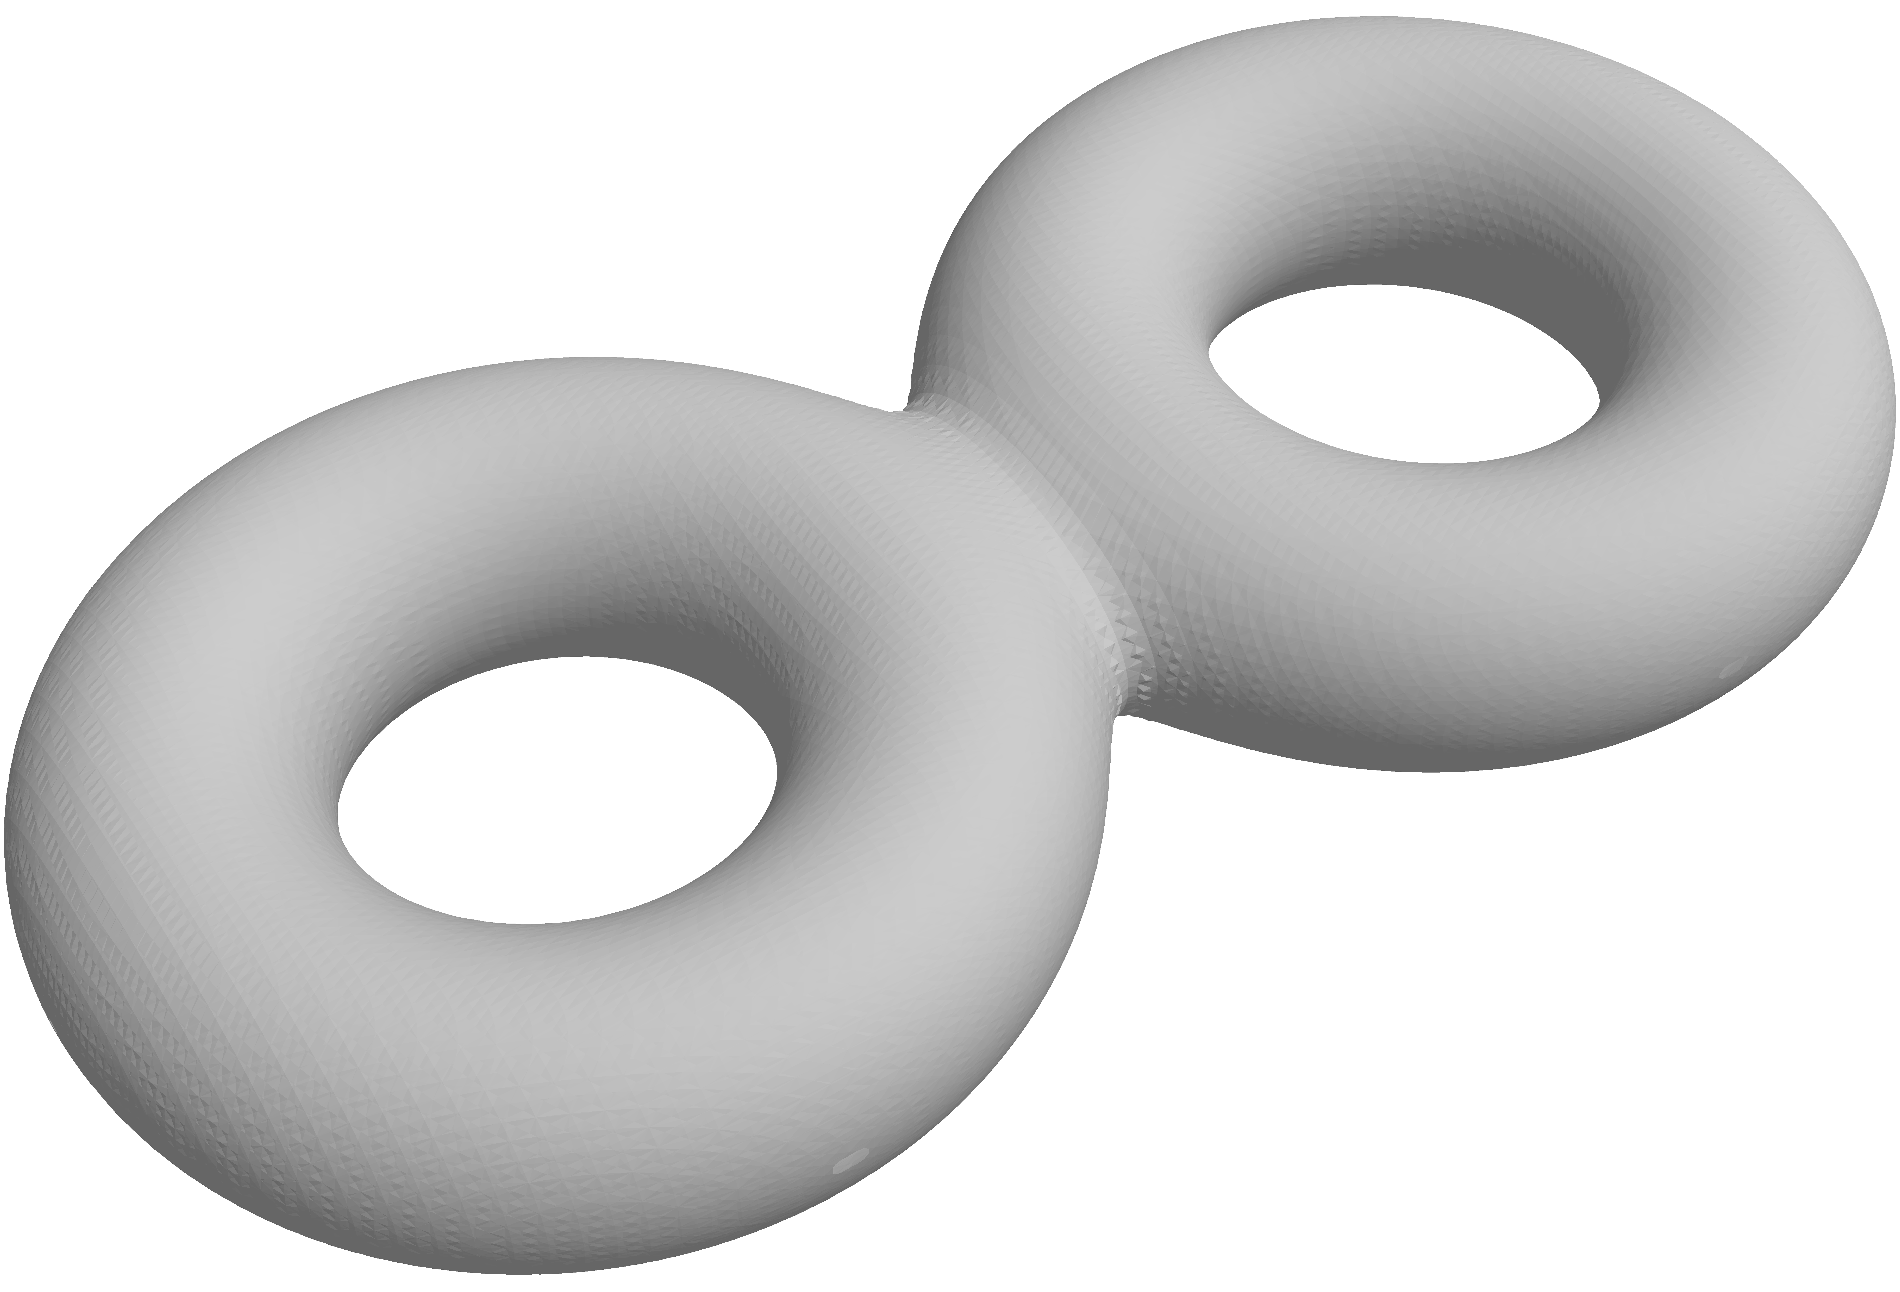
\includegraphics[width=5cm]{genus-2-surface}};
\end{tikzpicture}
\end{document}

\begin{example}
Take two tori, poke holes in them, and join together along a tube; let \(X\) be the resulting surface of genus \(2\).
Each punctured torus is an open set \(X_1, X_2 \subset X\), and the tube is their intersection \(X_0=X_1 \cap X_2\).
The tube \(X_0\) has fundamental group \(\pi_0=\Z{}\), and this includes into each fundamental group of each punctured torus as a small circle around the puncture.
On each torus, the circle around the puncture is the product \(xyx^{-1}y^{-1}\), which of course vanishes once we close up the puncture.
So if we glue two tori together, the resulting surface \(X\) of genus \(2\) has fundamental group 
\[
\left<x,y,X,Y|xyx^{-1}y^{-1}=XYX^{-1}Y^{-1}\right>.
\]
\end{example}
\begin{problem}{covering.spaces:compact.fg}
Prove that the fundamental group of any compact, path connected, and locally simply connected topological space is finitely presented.
\end{problem}


\section{Homotopy groups}
For any topological space \(X\) with marked point \(x_0\), and any \(n\ge 1\), let \(\homotopyGroup{n}{X,x_0}\) be the set of all continuous maps \([0,1]^n \to X\) taking every boundary point of \([0,1]^n\) to \(x_0\), modulo homotopy through such maps.
Each \(\homotopyGroup{n}{X,x_0}\) has a distinguished point: the constant map.

There is a special case: \(n=0\).
We define \(\homotopyGroup{0}{X,x_0}\) to be the set of all components of \(X\), with a special chosen component: that of \(x_0\).
Make \(\homotopyGroup{0}{X,x_0}\) into a topological space, by the quotient topology.

For \(n\ge 1\), take \(f,g \colon [0,1]^n \to X\) each mapping the boundary of \([0,1]^n\) to \(x_0\).
Define \(f*g\) to be the usual 
\[
(f*g)(t,x_2,\dots,x_n) =
\begin{cases}
f(2t,x_2,\dots,x_n), & \text{if \(0 \le t\le \frac{1}{2}\)}, \\
g(2t-1,x_2,\dots,x_n), & \text{if \(\frac{1}{2} \le t\le 1\)},
\end{cases}
\]
and \(\bar{f}(t,x_2,\dots,x_n)=f(1-t,x_2,\dots,x_n)\).
If \(f \colon X \to Y\) is continuous, and \(y_0\defeq f(x_0)\), define \(f_* \colon \homotopyGroup{*}{X,x_0} \to \homotopyGroup{*}{Y,y_0}\) by \(f_*[g] = [f \circ g]\).

A \emph{contraction}\define{contraction} of a topological space \(X\) to a point \(x_0\in X\) is a continuous map \(\varphi\colon X\times[0,1]\to X\) so that \(\varphi(x,0)=x\) and \(\varphi(x,1)=x_0\) for any \(x\in X\).
A topological space \(X\) is \emph{contractible}\define{contractible} if it has a contraction.
\begin{problem}{covering.space:contractible}
Prove that every contractible space is connected and has trivial homotopy groups.
\end{problem}
Given a continuous map \(f \colon X \to Y\), a \emph{lift}\define{lift} of a continuous map \(g \colon Z \to Y\) is a continuous map \(\hat{g} \colon Z \to X\) so that \(f \circ \hat{g}=g\).
A \emph{Serre fibration}\define{Serre fibration} is a continuous map \(f \colon X \to Y\) of topological spaces, so that for any box \(Z=[0,1]^n\) and continuous map \(g \colon Z \times [0,1] \to Y\), denoted \(g_t(z)\defeq g(z,t)\), every lift of \(g_0\) extends to a lift of \(g\).
\begin{theorem}
If \(f \colon X \to Y\) is a Serre fibration, then the obvious maps 
\[
\homotopyGroup{n}{F,x_0}\to\homotopyGroup{n}{X,x_0}\to\homotopyGroup{n}{Y,y_0}
\]
fit together into an exact sequence
\begingroup
\newcommand*{\xA}[1]{\homotopyGroup{#1}{F,x_0}}
\newcommand*{\xB}[1]{\homotopyGroup{#1}{X,x_0}}
\newcommand*{\xC}[1]{\homotopyGroup{#1}{Y,y_0}}
\reverseLongExactSequence{\xA}{\xB}{\xC}
\endgroup
\end{theorem}

Pick \(x_0 \in X\), let \(y_0\defeq f(x_0)\) and let \(F\defeq f^{-1}\set{y_0}\subseteq X\).
The morphism \(\fundamentalGroup{X,x_0}\to\fundamentalGroup{Y,y_0}\) kills loops in \(X\) which lie entirely in a fiber \(F=f^{-1}\set{y_0}\), i.e. those loops map to \(1\in\fundamentalGroup{Y,y_0}\).
More generally, it kills the loops in \(X\) which admit a homotopy, fixing endpoints, to a loop in \(F\).
Any loop in \(Y\) starting and ending at \(y_0\) lifts to a path in \(X\), starting at \(x_0\), but perhaps not a loop.
Since it is a loop in \(Y\), its lift has ends in \(X\) lying in the fiber \(F\).
Under homotopy of the loop in \(Y\), with fixed ends, the ends of the lift can only move inside \(F\), so they have well defined components, a map 
\[
\fundamentalGroup{X,x_0}\to\fundamentalGroup{Y,y_0}\to\homotopyGroup{0}{F,x_0},
\]
where \(\homotopyGroup{0}{X_{y_0},x_0}\) is the set of all path components of \(X_{y_0}\), and contains a distinguished element, the path component that contains \(x_0 \in X_{y_0}\).
If the ends of that lift lie in the same path component, then we can draw those two ends together, obtaining the path in \(Y\) from a path in \(X\), i.e. the image of the first map is the ``kernel'' of the second, i.e. the elements mapping to the distinguished component.

Take a continuous map \(h \colon Z \times [0,1] \to Y\), which we write as \(h_t(z)=h(z,t)\).
Suppose that \(h_0(z)=y_0\) for all \(z\), and \(h_s(z)=y_0\) for all \(z\in\partial Z\).
Lift \(h_0\) to the trivial map to \(x_0\).
Lift \(h\) to a map \(\hat{h} \colon Z \times [0,1] \to X\) extending that lift.
So \(f \circ \hat{h}_t(z)=h_t(z)\), and \(\hat{h}_0(z)=x_0\) for all \(z \in Z\).
Since \(h_s(z)=y_0\) for \(z \in \partial Z\), \(\hat{h}_s(z) \in F\) for \(z\in\partial Z\), for all \(s\).
In particular, \(\hat{h}_s(z)\) stays in the component of \(x_0\) in \(F\), for \(z\in\partial Z\), for all \(s\).
If we replace our choices at each step, still \(\hat{h}_1 \colon \partial Z \to F\) varies only by homotopy, giving an element of \(\homotopyGroup{n-1}{F,x_0}\), a map
\[
\homotopyGroup{n}{X,x_0}\to\homotopyGroup{n}{Y,y_0}\to\homotopyGroup{n-1}{F,x_0}.
\]
If this element vanishes, then \(\hat{h}_1\) is nulhomotopic in \(F\), and if we attach that homotopy to \(\hat{h}\), and its composition with \(X\to Y\) to \(h\), then \(h\) continues to map to \(h_s(z)=y_0\).
So \(h\) is an element of \(\homotopyGroup{n}{Y,y_0}\) arising from an element of \(\homotopyGroup{n}{X,x_0}\).
In other words, in
\[
\homotopyGroup{n}{X,x_0}\to\homotopyGroup{n}{Y,y_0}\to\homotopyGroup{n-1}{F,x_0}.
\]
 the kernel of the second map is the image of the first.

Being a Serre fibration is a local property in \(Y\):
\begin{lemma}\label{lemma:Serre.fibration.local}
A continuous map \(f \colon X \to Y\) of topological spaces is a Serre fibration if and only if there is an open cover of \(Y\) by open sets \(Y_a \subseteq Y\) so that, if \(X_a\defeq f^{-1}Y_a\) and \(f_a \defeq \left.f\right|_{X_a}\), then each \(f_a\) is a Serre fibration.
\end{lemma}
\begin{proof}
Take such an open cover, and some map \(g \colon Z \times [0,1] \to Y\) with a lift \(\hat{g}_0 \colon Z \to X\), where \(Z=[0,1]^n\).
Cover the image of \(g\) in our open sets \(Y_a\).
Take a finite subcover.
Divide up \(Z\times [0,1]\) into a grid of cubes small enough that each lies inside a single \(Y_a\).
Lift up one cube at a time.
\end{proof}
A \emph{projection}\define{projection map} is a map \((x,z)\in X \times Z\mapsto z \in Z\); the \emph{fiber} is \(Z\).
Two maps \(X_0 \to Y_0\) and \(X_1\to Y_1\) are \emph{isomorphic} if there are diffeomorphisms \(X_0 \to X_1\) and \(Y_0\to Y_1\)  making a commutative diagram
\begin{tikzcd}
X_0 \arrow{r} \arrow{d} & X_1 \arrow{d} \\
Y_0 \arrow{r} & Y_1
\end{tikzcd}
A continuous map is \emph{trivial} if isomorphic to a projection.
A continuous map \(\pi\colon X \to Y\) is \emph{locally trivial} ifevery point of \(Y\) lies in an open set \(U\subseteq Y\)  so that 
\[
\left.\pi\right|_{\pi^{-1}U}\colon \pi^{-1}U \to U
\]
is trivial.
A \emph{fiber bundle}\define{fiber bundle} is a continuous locally trivial map \(\pi\colon X \to Y\) of topological spaces.
\begin{lemma}
Every fiber bundle is a Serre fibration.
\end{lemma}
\begin{proof}
Fiber bundles are locally trivial, so true locally; apply lemma~\vref{lemma:Serre.fibration.local}.
\end{proof}
